\section{Numerical Results}
\label{sec:numerics}

This section presents numerical simulations that verify the
theoretical predictions and explore the practical performance of
stereographic block encoding.  All quantum circuit simulations
use the Qulacs library~\cite{Qulacs2021} (v0.6.13) for
statevector and density-matrix simulation; the
simulation code and data are available in the accompanying
repository.

\subsection{Heisenberg Model Verification}
\label{subsec:heisenberg-numerics}

We verify the stereographic block encoding of the two-qubit
Heisenberg model~\eqref{eq:heisenberg} by constructing the
full 3-qubit circuit (one ancilla plus two system qubits)
in Qulacs and comparing the decoded eigenvalue inversion
$f(\lambda') = 1/\lambda'$ with exact diagonalization.

The simulation sweeps over a grid of coupling and field
strengths $(J, h) \in \{0.5, 1, 2\} \times \{0, 0.25,
	0.5, 1, 2\}$ (15 parameter sets, 4 eigenstates each).
For each parameter set, we shift the spectrum to positive
values, find QSP phases at degree $d = 14$ for the target
$f(r) = 1/r$, build the uniformly-controlled signal
operator in the eigenbasis, and run the circuit.

Figure~\ref{fig:heisenberg-verification}(a) shows the
decoded circuit output versus the exact $1/\lambda'$ across
all 60 eigenstate--parameter combinations.  All points
lie on the identity line, confirming the circuit produces
the correct eigenvalue transformation.
Figure~\ref{fig:heisenberg-verification}(b) displays the
maximum error $|f_{\mathrm{decoded}} - 1/\lambda'|$ for
each $(J, h)$ pair as a heatmap.  The circuit--matrix
discrepancy (quantum circuit vs.\ classical 2$\times$2
matrix calculation at the same QSP phases) is uniformly
below $10^{-13}$, confirming that the circuit construction
is exact to machine precision.  The remaining error is the
QSP polynomial approximation error for $1/r$, which depends
on the degree and the eigenvalue range.

\begin{figure*}
	\centering
	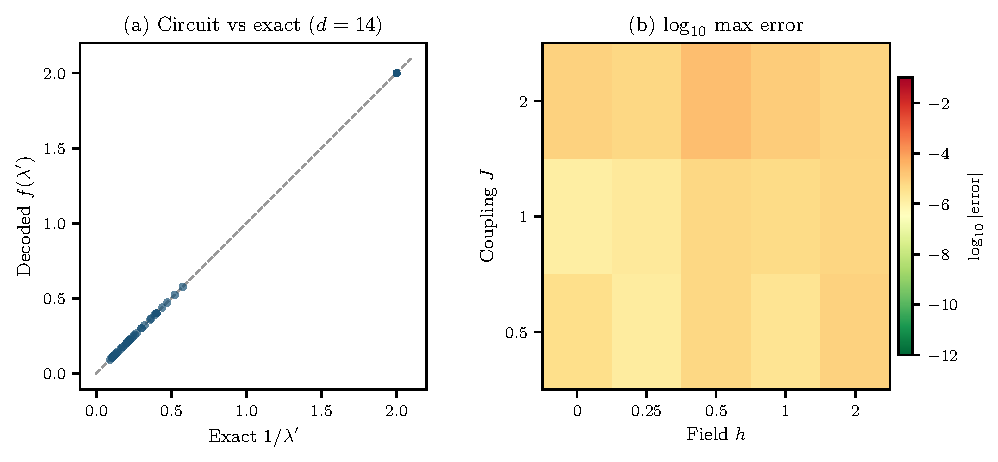
\includegraphics[width=\textwidth]{figures/heisenberg_verification.pdf}
	\caption{Verification of stereographic block encoding
		on the two-qubit Heisenberg model across 15 parameter
		sets.  (a) Decoded eigenvalue inversion from the quantum
		circuit versus exact $1/\lambda'$ for all eigenstates
		at QSP degree $d=14$.  (b) Heatmap of the maximum
		approximation error over eigenstates for each $(J, h)$
		combination.}
	\label{fig:heisenberg-verification}
\end{figure*}

\subsection{Gate Count Benchmarks}
\label{subsec:gate-counts}

We compare the resource requirements of stereographic block
encoding with standard block encoding (via LCU) for the three
Hamiltonian classes of Section~\ref{sec:circuits}.
Table~\ref{tab:gate-counts} summarizes the CNOT count,
single-qubit gate count, and ancilla requirements.

For diagonal Hamiltonians on $n$ qubits, stereographic
encoding uses $2^n$ CNOT and $2^n$ single-qubit gates
(from the uniformly controlled $R_y$), with a single
ancilla qubit and no normalization factor.  Standard LCU
encoding requires roughly $2 \times 2^n$ gates and
$\lceil \log_2 2^n \rceil = n$ ancilla qubits.  The
stereographic advantage in ancilla count is logarithmic
in the system dimension.

For Pauli-$Z$ sums with $m$ terms, stereographic encoding
uses $\mathcal{O}(m)$ gates via reversible arithmetic, scaling
with the number of terms rather than the Hilbert space
dimension.  The normalization factor $\alpha$ for standard
LCU grows as $\sum_k |c_k|$, directly inflating the QSVT
depth.

For the Heisenberg model, the stereographic circuit depth
is constant ($\sim\!23$ for $d = 10$) regardless of the
coupling strength $J$ or field $h$, because the Givens
rotation diagonalization has $\mathcal{O}(1)$ gate complexity.
The standard LCU approach requires depth proportional to
$\alpha = 3J + h$, which grows with the Hamiltonian norm.

\begin{table*}
	\caption{Gate count comparison for stereographic
		vs.\ standard block encoding at QSP degree $d = 10$.
		CNOT and single-qubit (1Q) gate counts are shown
		alongside ancilla qubit requirements and normalization
		factor $\alpha$.  For the Heisenberg model, circuit
		depth is reported instead of individual gate counts.}
	\label{tab:gate-counts}
	\begin{ruledtabular}
		\begin{tabular}{llcccccccc}
			           &                 & \multicolumn{4}{c}{Stereographic} & \multicolumn{4}{c}{Standard}                                                                           \\
			\hline
			Class      & Params          & CNOT                              & 1Q                           & Anc.\  & $\alpha$                      & CNOT & 1Q  & Anc.\  & $\alpha$ \\
			\hline
			Diagonal   & $n=2$           & 4                                 & 4                            & 1      & ---                           & 8    & 8   & 2      & 6.9      \\
			Diagonal   & $n=3$           & 8                                 & 8                            & 1      & ---                           & 16   & 16  & 3      & 9.9      \\
			Diagonal   & $n=4$           & 16                                & 16                           & 1      & ---                           & 32   & 32  & 4      & 17.7     \\
			Diagonal   & $n=5$           & 32                                & 32                           & 1      & ---                           & 64   & 64  & 5      & 43.8     \\
			$Z$-sum    & $m=2$           & 6                                 & 4                            & 1      & ---                           & 8    & 8   & 1      & 2        \\
			$Z$-sum    & $m=4$           & 12                                & 8                            & 1      & ---                           & 16   & 16  & 2      & 4        \\
			$Z$-sum    & $m=8$           & 24                                & 16                           & 1      & ---                           & 32   & 32  & 3      & 8        \\
			$Z$-sum    & $m=16$          & 48                                & 32                           & 1      & ---                           & 64   & 64  & 4      & 16       \\
			Heisenberg & $J{=}1,h{=}0$   & \multicolumn{2}{c}{depth 23}      & 1                            & ---    & \multicolumn{2}{c}{$\sim$200} & 2    & 3.0                     \\
			Heisenberg & $J{=}1,h{=}0.5$ & \multicolumn{2}{c}{depth 23}      & 1                            & ---    & \multicolumn{2}{c}{$\sim$200} & 2    & 3.5                     \\
			Heisenberg & $J{=}2,h{=}0.5$ & \multicolumn{2}{c}{depth 23}      & 1                            & ---    & \multicolumn{2}{c}{$\sim$200} & 2    & 6.5                     \\
		\end{tabular}
	\end{ruledtabular}
\end{table*}

\subsection{Eigenvalue Transformation Accuracy}
\label{subsec:transform-accuracy}

We apply the full stereographic QSVT protocol to compute
$f(\lambda) = 1/\lambda$ (eigenvalue inversion) on the
two-qubit Heisenberg model with $J = 1$, $h = 0.5$ and
study the convergence as the QSP degree $d$ increases.

For each degree $d \in \{2, 4, 6, \ldots, 28\}$, we find
the optimal QSP phases for $f(r) = 1/r$ using the
phase-finding algorithm of the companion
paper~\cite{KharaziLeytonOrtega2026a}, build the full
3-qubit circuit, and decode the eigenvalue transformation
from the ancilla.
Figure~\ref{fig:convergence}(a) shows the approximation
error $|f_{\mathrm{decoded}} - 1/\lambda'|$ versus the
QSP degree for each of the four eigenstates.  The error
decreases monotonically with degree, reaching
$\sim\!10^{-3}$ at degree $d = 28$.
Figure~\ref{fig:convergence}(b) shows the maximum error
across all eigenstates as a function of circuit depth,
confirming that accuracy improves steadily as depth
increases.

The convergence rate depends on the eigenvalue range:
eigenstates with $\lambda' \approx 0.5$ (the smallest
shifted eigenvalue, where $1/\lambda' = 2$) are hardest
to approximate because the target function is large and
steep there, while eigenstates with $\lambda' \approx 5$
converge more rapidly.  This is consistent with the
$1/r$ approximation theory from the companion paper.

\begin{figure*}
	\centering
	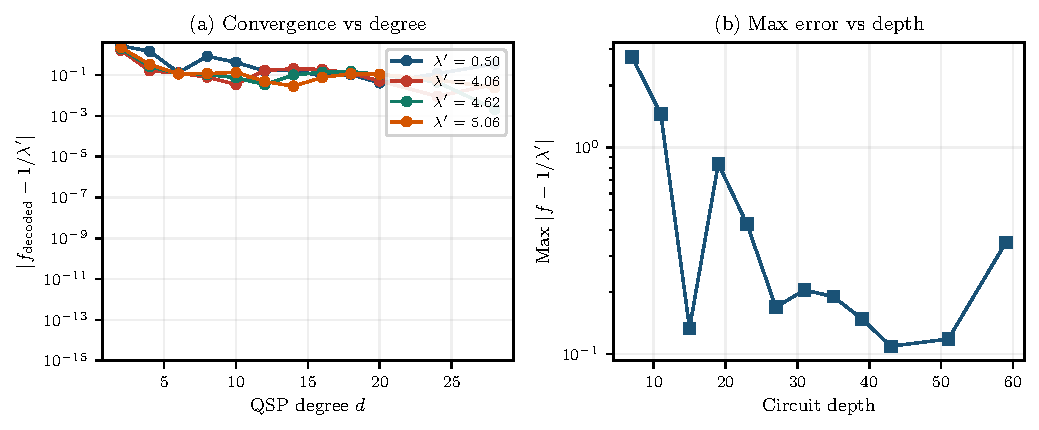
\includegraphics[width=\textwidth]{figures/convergence_vs_degree.pdf}
	\caption{Convergence of eigenvalue inversion for the
		Heisenberg model ($J=1$, $h=0.5$).
		(a)~Approximation error vs.\ QSP degree for each
		eigenstate.  (b)~Maximum error vs.\ circuit depth.}
	\label{fig:convergence}
\end{figure*}

\subsection{Noise Analysis}
\label{subsec:noise}

We analyze the sensitivity of stereographic block encoding
to two noise sources: finite measurement statistics
(shot noise) and coherent gate noise (depolarizing channel).

\emph{Sampling noise.}
In stereographic decoding, the rational function
$f(\lambda) = (\langle X \rangle + i \langle Y \rangle)
	/ (1 - \langle Z \rangle)$ is reconstructed from three
Pauli expectation values on the ancilla.  Each expectation
has variance $(1 - \langle P \rangle^2)/N$ for $N$
measurement shots.  We simulate this by adding Gaussian
noise with the appropriate variance to the exact Pauli
expectations obtained from the statevector.
Figure~\ref{fig:noise}(a) shows the mean decoded error
versus shot count $N$ for each eigenstate.  The statistical
uncertainty decreases as $1/\sqrt{N}$, as expected.

The total shot overhead depends on the stereographic
parameter $r = \lambda'$ through the Bloch vector
geometry.  For large $r$, the Bloch vector approaches
the south pole ($\langle Z \rangle \to -1$, $\langle X
	\rangle, \langle Y \rangle \to 0$), and the decoding
formula has a benign denominator $1 - \langle Z \rangle
	\approx 2$.  For small $r$, the Bloch vector approaches
the north pole ($\langle Z \rangle \to 1$), and the
denominator $1 - \langle Z \rangle \ll 1$ amplifies
noise, giving the $\mathcal{O}(r^6/\epsilon^2)$ scaling
of Section~\ref{sec:decoding}.

\emph{Gate noise.}
We add depolarizing noise with rate $p$ after each gate
in the circuit and simulate the resulting density matrix
evolution in Qulacs.
Figure~\ref{fig:noise}(b) shows the decoded error versus
depolarizing rate for two representative eigenstates.
For noise rates below $10^{-3}$, the error is dominated
by the QSP polynomial approximation; above $10^{-3}$,
gate noise degrades the decoded output approximately
linearly in $p$.  The stereographic circuit's reduced
depth (compared to standard QSVT with normalization-inflated
depth) provides a natural advantage in the noisy regime:
fewer gates means less accumulated noise.

\begin{figure*}
	\centering
	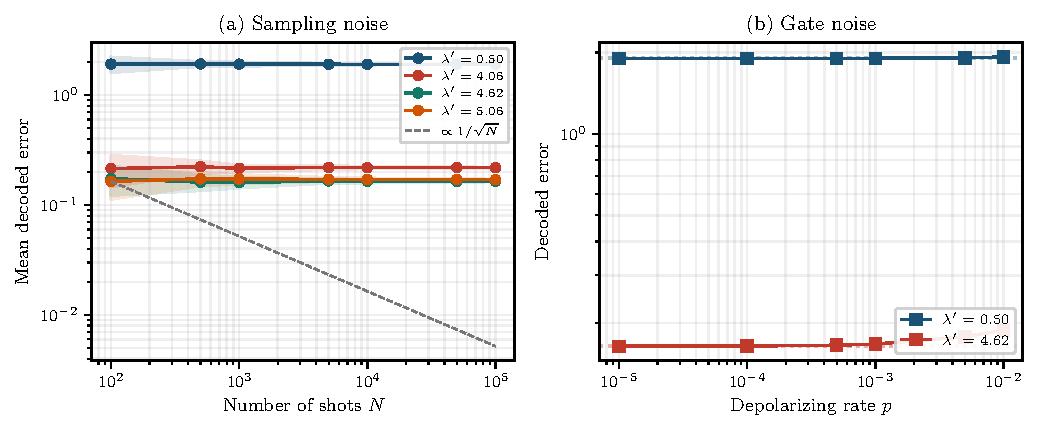
\includegraphics[width=\textwidth]{figures/noise_analysis.pdf}
	\caption{Noise analysis for stereographic block encoding
		of the Heisenberg model ($J=1$, $h=0.5$, $d=14$).
		(a)~Mean decoded error vs.\ number of measurement
		shots, with shaded bands showing $\pm 1\sigma$
		over 50 repetitions.  The dashed line shows
		$1/\sqrt{N}$ scaling.
		(b)~Decoded error vs.\ depolarizing noise rate
		for two eigenstates.  Dashed lines show the
		noiseless baseline.}
	\label{fig:noise}
\end{figure*}
